\documentclass[11pt,a4paper]{article}
\usepackage[utf8]{inputenc}
\usepackage[T1]{fontenc}
\usepackage{amsmath,amssymb}
\usepackage{graphicx}
\usepackage{booktabs}
\usepackage[margin=25mm]{geometry}
\usepackage[colorlinks=true,linkcolor=blue,citecolor=blue,urlcolor=blue]{hyperref}

\newcommand{\vect}[1]{\mathbf{#1}}
\newcommand{\uv}[1]{\hat{\mathbf{#1}}}
\newcommand{\Ms}{M_\mathrm{s}}
\newcommand{\HB}{H_\mathrm{B}}
\newcommand{\dd}{\mathrm{d}}
\newcommand{\ee}{\mathrm{e}}
\newcommand{\ii}{\mathrm{i}}

\title{Analytical model of the self-generated standing spin wave\\
in the orthogonal biquadratic-coupled spin-torque oscillator\\[4pt]
\large Detailed derivation}
\author{Notes accompanying \texttt{APL\_figures/standing\_wave\_theory}}
\date{September 2026}

\begin{document}
\maketitle

\begin{abstract}
The micromagnetic simulations of the CoPt/Cr/CoFe orthogonal spin-torque oscillator (STO) show, on top of the
in-plane gyration of the free layer, an out-of-plane ($M_z$) pattern of concentric rings and a one-armed spiral
phase map at the gyration frequency, together with a staircase in the frequency-versus-current relation.
This note derives, step by step, an analytical description of that pattern.  The central results are
(i) in a frame that rotates in \emph{spin space} together with the gyrating magnetisation the free layer is an
in-plane film with zero internal field, whose small excitations follow the ordinary dipole--exchange dispersion
$\Omega(k)$; (ii) the static, axisymmetric stray field of the perpendicular fixed layer is, in that frame, a
microwave drive at the gyration frequency $\omega$ with azimuthal index $m=1$, so that it launches an inward
spiral spin wave with the wavenumber $k^\ast$ fixed by the selection rule $\Omega(k^\ast)=\omega$;
(iii) regularity at the disk centre turns the wave into a $J_1(k^\ast r)\,\ee^{\ii\phi}$ standing pattern whose
radial phase $k^\ast R$ is pinned, plateau by plateau, close to the zeros of $J_1$; this gives the ladder of plateau
frequencies $f_n=\Omega(x_n/R)/2\pi$ and the step height $\Delta f\simeq(\partial\Omega/\partial k)/2R$;
(iv) the diameter dependence follows from the same picture: the frequency is the macrospin frequency reduced by
the power stored in the wave, $f=f_\mathrm{mac}/(1+\beta\langle a^2\rangle)$, the sawtooth is the oscillator hopping
between successive cavity modes, and the steps fade once the disk radius exceeds the damping length of the wave.
Without any fitted parameter the selection rule reproduces the simulated gyration frequency from the measured
wavenumber to $7\pm8\,\%$ over 177 runs (8--35\,GHz, with and without biquadratic coupling, current and diameter
sweeps), and the plateau ladder is bracketed to within 1--2\,GHz.
\end{abstract}

\tableofcontents

\section{What the simulation maps contain}
\label{sec:maps}

Before deriving anything it is worth stating precisely what the per-cell FFT maps show, because the
description in the manuscript draft (``4 rings, spiral of 4 rotations'') is not what the data contain.
Table~\ref{tab:maps} summarises the analysis of the complex FFT maps at the gyration frequency
(\texttt{heat\_map.npy}) for the two reference runs, $D=320$\,nm, $J=6.0$ (with BQ) and $5.5\times10^{11}$\,A/m$^2$
(without BQ).  The map $X(r,\phi)$ was decomposed into azimuthal harmonics,
$X=\sum_m X_m(r)\,\ee^{\ii m\phi}$, and the radial phase of the dominant harmonic was unwrapped.

\begin{table}[h]
\centering
\caption{Content of the $M_z$ FFT maps at the gyration frequency ($R=160$\,nm).}
\label{tab:maps}
\begin{tabular}{lcc}
\toprule
 & with BQ (13.1\,GHz) & without BQ (12.0\,GHz)\\
\midrule
dominant azimuthal harmonic & $|m|=1$ (97\,\% of power) & $|m|=1$ (98\,\%)\\
radial wavelength $\lambda=2\pi/k$ (phase slope) & 94\,nm & 92\,nm\\
amplitude maxima along a radius & $r\simeq28,\,78,\,123$\,nm, rim & $25,\,78,\,123$\,nm, rim\\
amplitude minima & $55,\,100,\,143$\,nm & $55,\,100,\,143$\,nm\\
total phase winding, centre to rim & 1.5 turns & 1.3 turns\\
\bottomrule
\end{tabular}
\end{table}

With $k=2\pi/94\,\mathrm{nm}=0.067\,\mathrm{nm}^{-1}$ the zeros of the Bessel function $J_1(kr)$,
$kr=3.83,\,7.02,\,10.17$, fall at $r=57,\,105,\,152$\,nm and its extrema, $kr=1.84,\,5.33,\,8.54$, at
$r=27,\,80,\,127$\,nm, in agreement with the measured minima and maxima.  The pattern is therefore a
$J_1(kr)\,\ee^{\ii\phi}$ standing wave.  Its amplitude rings are spaced by $\lambda/2$, the ``four rings'' are the
three interior antinodes plus the rim antinode, and the phase map is a staircase with a step of $\pi$ at every
node (the standing part) superposed on a slow drift (a residual inward-propagating part), which the eye reads
as a spiral.  Everything below is built to explain this pattern and the value of $k$.

\section{Model and conventions}
\label{sec:model}

\subsection{Equation of motion}
The simulator (magnum.np) integrates the Landau--Lifshitz--Gilbert equation in the form
\begin{equation}
\frac{\partial\vect m}{\partial t}=-\gamma\,\vect m\times\vect H_\mathrm{eff}
+\alpha\,\vect m\times\frac{\partial\vect m}{\partial t},
\qquad \gamma=2.211\times10^{5}\ \mathrm{m\,A^{-1}s^{-1}},
\label{eq:llg}
\end{equation}
with all fields in A/m, so that a field $H$ produces the angular frequency $\omega=\gamma H$
($\gamma/2\pi=28.0$\,GHz per tesla of $\mu_0H$).  Free-layer parameters:
$\Ms=1.35\times10^{6}$\,A/m, $A=1.3\times10^{-11}$\,J/m, thickness $d=2$\,nm, $\alpha=0.035$,
$K_u=2.362\times10^{3}$\,J/m$^3$ (anisotropy field $2K_u/\mu_0\Ms=2.78$\,kA/m, i.e.\ 3.5\,mT in $\mu_0H$, neglected below), disk radius $R=160$\,nm.

\subsection{Effective fields}

\paragraph{Exchange.}
$\vect H_\mathrm{ex}=D\,\nabla^2\vect m$ with
\begin{equation}
D=\frac{2A}{\mu_0\Ms}=1.53\times10^{-11}\ \mathrm{A\,m}.
\end{equation}
For a plane wave $\ee^{\ii\vect k\cdot\vect r}$ this is a stiffness field $Dk^2$ acting on both transverse
components.

\paragraph{Demagnetising field of a thin film.}
For a uniform film $\vect H_\mathrm{d}=-\Ms m_z\uv z$.  For a magnetisation wave with in-plane wavevector
$\vect k$, averaged over the thickness $d$ (Kalinikos--Slavin lowest mode, unpinned surfaces), the dynamic dipolar
field is
\begin{equation}
\delta\vect H_\mathrm{d}(\vect k)=-\Ms\Big[P(kd)\,(\delta\vect m\cdot\uv z)\,\uv z
+\big(1-P(kd)\big)\,(\delta\vect m\cdot\uv k)\,\uv k\Big],
\qquad P(x)=\frac{1-\ee^{-x}}{x}.
\label{eq:dip}
\end{equation}
$P\to1$ at $k\to0$ (only the out-of-plane component is demagnetised), while at finite $k$ part of the
demagnetisation is transferred from the out-of-plane component to the in-plane component parallel to $\vect k$.
For small $kd$, $P\simeq1-kd/2$.

\paragraph{Biquadratic interlayer coupling.}
The simulator implements the areal energy $E_\mathrm{bq}=-B_{12}(\vect m_1\cdot\vect m_2)^2$ with
$B_{12}=-0.6$\,mJ/m$^2$, giving on the free layer (index 1, partner $\vect m_2$)
\begin{equation}
\vect H_\mathrm{bq}=-\frac{1}{\mu_0\Ms d}\frac{\partial E_\mathrm{bq}}{\partial\vect m_1}
=\frac{2B_{12}}{\mu_0\Ms d}\,(\vect m_1\cdot\vect m_2)\,\vect m_2 .
\end{equation}
With the fixed layer along $\uv z$ ($\vect m_2\simeq\uv z$) this is
\begin{equation}
\vect H_\mathrm{bq}=-\HB\,m_z\,\uv z,\qquad
\HB=\frac{2|B_{12}|}{\mu_0\Ms d}=3.54\times10^{5}\ \mathrm{A/m}\quad(\mu_0\HB=0.444\ \mathrm{T}).
\label{eq:HB}
\end{equation}
Because $B_{12}<0$ favours a perpendicular arrangement, the biquadratic field has exactly the same structure as
the demagnetising field of the film: it is an additional easy-plane stiffness.  Everywhere below $\Ms$ appears
as the out-of-plane stiffness it is accompanied by $\HB$ when the biquadratic coupling is switched on.

\paragraph{Spin-transfer torque.}
The Slonczewski torque is implemented as the field
\begin{equation}
\vect H_\mathrm{stt}=a_J\,\vect m\times\vect p,\qquad
a_J=\frac{\hbar J}{e\mu_0\Ms d}\,\epsilon,\qquad
\epsilon=\frac{P\Lambda^2}{(\Lambda^2+1)+(\Lambda^2-1)\,\vect m\cdot\vect p}\;\xrightarrow{\Lambda=1}\;\frac{P}{2},
\end{equation}
so that with $\Lambda=1$ the efficiency is independent of the angle between $\vect m$ and $\vect p$
(this will matter in Sec.~\ref{sec:frame}).  Inserting in Eq.~\eqref{eq:llg},
\begin{equation}
-\gamma\,\vect m\times\vect H_\mathrm{stt}=-\gamma a_J\,\vect m\times(\vect m\times\vect p)
=\gamma a_J\big[\vect p-(\vect m\cdot\vect p)\,\vect m\big].
\label{eq:stt}
\end{equation}
The polariser is $\vect p=(0,0.01,0.99)\simeq\uv z$; the 0.6$^\circ$ tilt is neglected.

\paragraph{Stray field of the fixed layer.}
The perpendicularly magnetised fixed layer produces at the free layer a static, axisymmetric field
$\vect h(r)=h_r(r)\,\uv r+h_z(r)\,\uv z$.  Inside the disk $h_z$ is small and positive (parallel to the fixed
layer's magnetisation) and $h_r$ is concentrated within roughly 15\,nm of the rim, where it produces the
up-tilted edge textures seen in the relaxed states.  This field is the \emph{source} of the spin wave
(Sec.~\ref{sec:source}); it is not needed for the dispersion.

\section{The gyrating state (macrospin)}
\label{sec:macrospin}

Let the free layer rotate rigidly in-plane with a constant tilt,
\begin{equation}
\vect m(t)=\big(\cos\theta_0\cos\Phi,\ \cos\theta_0\sin\Phi,\ \sin\theta_0\big),\qquad
\Phi=\omega_f t,\qquad m_{z0}=\sin\theta_0 .
\label{eq:opp}
\end{equation}
For this motion $\partial_t\vect m=\omega_f\,\uv z\times\vect m$ exactly.
The conservative fields are all along $\uv z$: $\vect H_\mathrm{d}+\vect H_\mathrm{bq}=-(\Ms+\HB)m_{z0}\uv z\equiv H_z\uv z$.
Writing $m_+=m_x+\ii m_y$ the precession part of Eq.~\eqref{eq:llg} gives
\begin{equation}
\dot m_+=\ii\gamma H_z\,m_+\quad\Longrightarrow\quad
\omega_f=\gamma H_z=-\gamma(\Ms+\HB)\,m_{z0}.
\label{eq:omegaf}
\end{equation}
A positive tilt therefore gyrates \emph{clockwise} (seen from $+z$); this is what the simulation does
($\omega_f/2\pi=-13.09$\,GHz with BQ, $-11.93$\,GHz without, measured from the last 5\,ns of the runs).

The dissipative torques must cancel separately.  Using Eq.~\eqref{eq:opp} in the Gilbert term,
\begin{equation}
\alpha\,\vect m\times\partial_t\vect m=\alpha\omega_f\,\vect m\times(\uv z\times\vect m)
=\alpha\omega_f\big[\uv z-m_z\vect m\big],
\end{equation}
which has the same vector structure as the spin-transfer torque \eqref{eq:stt} with $\vect p=\uv z$.
Their sum vanishes when
\begin{equation}
\alpha\omega_f+\gamma a_J=0\qquad\Longrightarrow\qquad
|\omega_f|=\frac{\gamma a_J}{\alpha},\qquad
m_{z0}=\frac{a_J}{\alpha(\Ms+\HB)} .
\label{eq:balance}
\end{equation}
Equations \eqref{eq:omegaf}--\eqref{eq:balance} are the familiar out-of-plane-precession (OPP) macrospin result:
the frequency is set by the balance between spin-transfer input and damping, the tilt adjusts so that the
easy-plane field produces that frequency, and the biquadratic coupling raises the frequency for a given tilt by
the factor $(\Ms+\HB)/\Ms=1.26$.  In the disk the frequency is lower than \eqref{eq:balance} because energy is
also lost to the spin wave; we therefore take $\omega\equiv|\omega_f|$ from the simulation and only use
\eqref{eq:omegaf} to relate tilt and frequency.  (With the fixed layer's stray field included,
$\omega=\gamma[(\Ms+\HB)m_{z0}-h_z]$; the measured tilts, 0.26 and 0.28, versus the values 0.22 and 0.25 given
by \eqref{eq:omegaf}, correspond to $\mu_0h_z\simeq0.05$--$0.09$\,T.)

\section{The co-rotating spin frame}
\label{sec:frame}

\subsection{Transformation}
The gyration is a rotation of the magnetisation \emph{vectors}, identical in every cell; the spatial pattern does
not move.  We therefore rotate spin space only, leaving the coordinates $(r,\phi)$ untouched:
\begin{equation}
\vect m(\vect r,t)=\mathsf R_z(\Phi)\,\vect m'(\vect r,t),\qquad \Phi=\omega_f t,
\label{eq:rot}
\end{equation}
where $\mathsf R_z(\Phi)$ is the rotation matrix about $\uv z$.  Two consequences follow immediately and are the key
to the whole problem:
\begin{enumerate}
\item $m_z$ is invariant: $m_z(\vect r,t)=m'_z(\vect r,t)$.  A wave $m'_z\propto\ee^{\ii(m\phi-\Omega t)}$ in the
rotating frame has \emph{the same} azimuthal index $m$, wavenumber and frequency $\Omega$ in the laboratory.
There is no Doppler shift for $m_z$.
\item The in-plane components mix with $\ee^{\pm\ii\Phi}$: $m_+=\ee^{\ii\omega_f t}m'_+$.  A field that is static in
the laboratory becomes, in the rotating frame, a field rotating at $-\omega_f$, i.e.\ a microwave field at the
gyration frequency.
\end{enumerate}

Since $\partial_t\vect m=\mathsf R_z(\partial_t\vect m'+\omega_f\uv z\times\vect m')$, and since exchange,
thin-film demagnetisation and the biquadratic field are all invariant under rotations about $\uv z$
(they transform covariantly, $\vect H'=\mathsf R_z^{-1}\vect H$), Eq.~\eqref{eq:llg} becomes
\begin{equation}
\partial_t\vect m'=-\gamma\,\vect m'\times\Big(\vect H'_\mathrm{eff}-\frac{\omega_f}{\gamma}\uv z\Big)
+\alpha\,\vect m'\times\partial_t\vect m'
+\big(\alpha\omega_f+\gamma a_J\big)\big[\uv z-m'_z\vect m'\big].
\label{eq:llgrot}
\end{equation}
Here $-\omega_f\uv z\times\vect m'=-\gamma\,\vect m'\times(-\omega_f\uv z/\gamma)$ has been written as a fictitious
field, the polariser $\vect p=\uv z$ is unchanged by the rotation, and the last term collects the damping of the
rigid rotation and the spin-transfer torque.

\subsection{The gyrating state is a zero-field equilibrium}
With the macrospin balance \eqref{eq:balance} the last term of \eqref{eq:llgrot} vanishes \emph{identically},
for any $\vect m'$, uniform or not: the spin torque exactly compensates the damping of the rotation everywhere,
and because $\epsilon$ does not depend on $\vect m\cdot\vect p$ for $\Lambda=1$ there is no residual angular
dependence.  What remains is a conservative LLG equation with the effective field
\begin{equation}
\vect H'_\mathrm{eff}-\frac{\omega_f}{\gamma}\uv z
=\vect H_\mathrm{ex}+\vect H_\mathrm{d}+\vect H_\mathrm{bq}+\big(\Ms+\HB\big)m_{z0}\,\uv z .
\end{equation}
For the uniform state $\vect m'_0=(\cos\theta_0,0,\sin\theta_0)$ the last three terms cancel by
Eq.~\eqref{eq:omegaf}: \emph{the total static field in the rotating frame is zero}.  The gyrating STO is, in
its own spin frame, a static in-plane film with no internal field at all; the only static energy is the
easy-plane stiffness that resists changes of $m'_z$.

\subsection{Why the frequency of the pattern is $\omega$}
Two remarks that remove the paradox which usually blocks this analysis.  (a) Because only spin space is rotated,
the frame does \emph{not} change the frequency or the azimuthal index of an $m_z$ pattern, so a
rotating-frame wave at $\Omega$ appears at $\Omega$ in the laboratory, whatever its azimuthal index.  (b) A static
texture in the rotating frame ($\Omega=0$ at $k\neq0$) is impossible: the linearised static problem has the
positive-definite stiffness of Sec.~\ref{sec:disp} and the uniform state is a strict energy minimum (up to the
global in-plane rotation).  Hence an $m_z$ pattern observed at the gyration frequency is a genuine spin wave of
the zero-field film at that frequency, and its wavenumber must lie on the dispersion curve $\Omega(k)=\omega$.

\section{Linear spin waves of the gyrating state}
\label{sec:disp}

\subsection{Linearisation}
Let $\vect m'=\vect m'_0+\delta\vect m$ with $\delta\vect m=a\,\uv e_1+b\,\uv e_2$ in the tangent frame
\begin{equation}
\begin{aligned}
&\uv e_1=\uv y\ \ (\text{in-plane, transverse}),\qquad
\uv e_2=(-\sin\theta_0,\,0,\,\cos\theta_0)\ \ (\text{polar}),\\
&\vect m'_0\times\uv e_1=\uv e_2,\qquad \vect m'_0\times\uv e_2=-\uv e_1 .
\end{aligned}
\end{equation}
Because the static field vanishes, the undamped linearised equation is simply
$\partial_t\delta\vect m=-\gamma\,\vect m'_0\times\delta\vect H$.
For a plane wave $\propto\ee^{\ii(\vect k\cdot\vect r-\Omega t)}$ every field term is linear,
$\delta\vect H=-\mathsf N\,\delta\vect m$, where the $2\times2$ stiffness matrix $\mathsf N$ (in A/m) collects:
\begin{align}
\text{exchange:}&\qquad N_{11}=N_{22}=Dk^2,\\
\text{biquadratic:}&\qquad \delta\vect H_\mathrm{bq}=-\HB\,\delta m_z\uv z=-\HB\,b\cos\theta_0\,\uv z
\ \Rightarrow\ N_{22}=\HB\cos^2\theta_0,\\
\text{dipolar, Eq.~\eqref{eq:dip}:}&\qquad
N_{11}=\Ms(1-P)\sin^2\varphi_k,\nonumber\\
&\qquad N_{22}=\Ms\big[P\cos^2\theta_0+(1-P)\sin^2\theta_0\cos^2\varphi_k\big],\nonumber\\
&\qquad N_{12}=N_{21}=-\Ms(1-P)\sin\theta_0\sin\varphi_k\cos\varphi_k ,
\end{align}
with $\varphi_k$ the angle between $\vect k$ and the in-plane direction of $\vect m'_0$
(we used $\uv e_1\cdot\uv k=\sin\varphi_k$, $\uv e_2\cdot\uv k=-\sin\theta_0\cos\varphi_k$,
$\uv e_2\cdot\uv z=\cos\theta_0$).  Projecting $\partial_t\delta\vect m=\gamma\,\vect m'_0\times(\mathsf N\delta\vect m)$
on $\uv e_1,\uv e_2$:
\begin{equation}
\dot a=-\gamma\,(N_{21}a+N_{22}b),\qquad \dot b=\gamma\,(N_{11}a+N_{12}b),
\end{equation}
and with $\partial_t\to-\ii\Omega$,
\begin{equation}
\boxed{\;\Omega^2=\gamma^2\big(N_{11}N_{22}-N_{12}^2\big)\;}
\label{eq:Omega2}
\end{equation}
the Smit--Beljers form with zero static field.

\subsection{Dispersion for a radial wave}
The wave of interest propagates radially, so $\varphi_k$ runs through all values around the disk while
$\vect m'_0$ is fixed.  The one-armed mode is not an eigenmode of the anisotropic $\varphi_k$-dependent problem but
of its azimuthal average; we therefore replace $\sin^2\varphi_k,\cos^2\varphi_k\to\tfrac12$ and drop the cross term
$N_{12}^2$, which is of order $(1-P)^2\sin^2\theta_0$ (below 1\,\%).  The result is
\begin{equation}
\boxed{\;\begin{aligned}
\Omega(k)^2=\gamma^2&\Big[Dk^2+\tfrac12\Ms\big(1-P(kd)\big)\Big]\\
\times&\Big[Dk^2+\big(\Ms P(kd)+\HB\big)\cos^2\theta_0+\tfrac12\Ms\big(1-P(kd)\big)\sin^2\theta_0\Big]
\end{aligned}\;}
\label{eq:disp}
\end{equation}
with $\sin\theta_0=m_{z0}=\omega/[\gamma(\Ms+\HB)]$ from Eq.~\eqref{eq:omegaf}.
The first bracket is the in-plane (``phase'') stiffness: it vanishes at $k=0$, the Goldstone mode of the
oscillator (a global shift of the gyration phase costs nothing), and grows through exchange and the in-plane
dipolar term.  The second bracket is the out-of-plane (``tilt'') stiffness, dominated by $\Ms P+\HB$; this is
where the biquadratic coupling enters and stiffens the wave.

\paragraph{Limits.}
For small $kd$, $1-P\simeq kd/2$.  When exchange dominates the first bracket ($Dk^2\gg\Ms kd/4$, i.e.\
$k\gg\Ms d/4D\simeq44\ \mu\mathrm{m}^{-1}$) the dispersion is linear,
\begin{equation}
\Omega\simeq c\,k,\qquad c=\gamma\sqrt{D(\Ms+\HB)}\cos\theta_0
=\begin{cases}1006\ \mathrm{m/s}\cos\theta_0 & \text{no BQ}\\ 1130\ \mathrm{m/s}\cos\theta_0 & \text{BQ,}\end{cases}
\label{eq:sound}
\end{equation}
the ``spin-superfluid sound'' velocity of an easy-plane magnet.  In the range actually used by the STO
($k=40$--$200\ \mu\mathrm{m}^{-1}$, $kd=0.08$--$0.4$) the in-plane dipolar term is comparable to exchange, which
makes $\Omega(k)$ slightly concave and shifts it upward; Eq.~\eqref{eq:disp} rather than \eqref{eq:sound}
is used for all numbers below.  Note that the exchange-only guess $\Omega=\gamma Dk^2$ (which is what one obtains
by ignoring the easy-plane stiffness) is 3--10 times too small in this range.

\section{The source: the fixed-layer stray field seen from the rotating frame}
\label{sec:source}

The stray field $\vect h(r)=h_r(r)\uv r+h_z(r)\uv z$ of the fixed layer is static and axisymmetric in the
laboratory.  Its in-plane part, written in Cartesian components, is $h_r(\cos\phi,\sin\phi,0)$; in the rotating
spin frame it becomes $\mathsf R_z^{-1}(\Phi)\vect h=h_r\big(\cos(\phi-\omega_f t),\sin(\phi-\omega_f t),0\big)$.
Its components along the two transverse directions of the equilibrium are
\begin{equation}
h'_1=\vect h'\cdot\uv e_1=h_r(r)\,\sin(\phi-\omega_f t),\qquad
h'_2=\vect h'\cdot\uv e_2=-\sin\theta_0\,h_r(r)\,\cos(\phi-\omega_f t).
\label{eq:drive}
\end{equation}
In the frame where the medium is static, the rim therefore carries a transverse microwave field
\emph{at the gyration frequency} with azimuthal dependence $\ee^{\ii(\phi-\omega_f t)}$: azimuthal index $m=1$,
rotating in the same sense as the magnetisation.  Physically: the torque the edge field exerts on the rotating
moment is largest where $\uv r\perp\vect m$, and that place travels around the rim once per gyration period.
The $z$ component $h_z$ is axisymmetric and static in both frames and only renormalises the tilt.

The medium being linear and axisymmetric (after the azimuthal averaging of Sec.~\ref{sec:disp}), the response has
the same $(\phi,t)$ dependence as the drive,
\begin{equation}
\delta\vect m(r,\phi,t)=\mathrm{Re}\big[\vect u(r)\,\ee^{\ii(\phi-\omega_f t)}\big],\qquad
m_z-m_{z0}=\cos\theta_0\,\mathrm{Re}\big[u_2(r)\,\ee^{\ii(\phi-\omega_f t)}\big],
\end{equation}
and, away from the rim where the drive vanishes, $\vect u(r)$ satisfies the free wave equation in polar
coordinates with $\nabla^2\to\partial_r^2+r^{-1}\partial_r-r^{-2}$ (the $m=1$ Laplacian) at frequency
$\Omega=\omega$.  The radial wavenumber is therefore fixed by the
\begin{equation}
\boxed{\ \text{selection rule:}\qquad \Omega(k^\ast)=\omega\ }
\label{eq:selection}
\end{equation}
where $\omega=|\omega_f|$ is the gyration frequency itself.  This is the quantitative content of the statement
``the spin wave propagates at the same frequency as the in-plane oscillation'': the frequency is that of the
gyration, and the wavelength is whatever the zero-field dispersion assigns to that frequency.

Two checks against the raw data.  First, the handedness: Eq.~\eqref{eq:drive} predicts an $m_z$ pattern whose
phase is constant on $\phi=\omega_f t$, i.e.\ co-rotating with the magnetisation.  The last 5\,ns of the two
reference runs give a co-rotating $|m|=1$ component with 100 times the power of the counter-rotating one
(218 vs 2.0 with BQ, 406 vs 2.4 without, arbitrary units), an $m=0$ ring component below 0.2\,\%, no static spiral
in the time-averaged $m_z$, and a second harmonic ($m=2$ at $2\omega$) at 8\,\% of the fundamental power,
consistent with the large wave amplitude ($\delta m_z\simeq0.17$).  Second, the local gyration rate is uniform
across the disk to within 3\,\%, so a single $\omega_f$ describes the whole disk and the frame transformation is
legitimate.

\section{Standing wave in the disk and the frequency staircase}
\label{sec:cavity}

\subsection{Radial mode shape}
Regularity at $r=0$ of an $m=1$ solution of the Helmholtz equation selects the Bessel function,
\begin{equation}
u_2(r)\propto J_1(k^\ast r)\quad\text{(plus, with damping, a small inward-travelling admixture)},
\end{equation}
so the $m_z$ pattern is
\begin{equation}
m_z(r,\phi,t)-m_{z0}\simeq A\,J_1(k^\ast r)\cos(\phi-\omega_f t+\delta).
\label{eq:pattern}
\end{equation}
Its FFT amplitude at $\omega$ is $\propto|J_1(k^\ast r)|$: rings at the extrema of $J_1$, minima at its zeros,
i.e.\ spaced by $\lambda/2$, and its phase jumps by $\pi$ at every zero.  With a small propagating admixture the
jumps are rounded into the observed staircase-spiral.  Equation~\eqref{eq:pattern} with
$k^\ast=0.067$--$0.070\,\mathrm{nm}^{-1}$ reproduces every node and antinode position of Table~\ref{tab:maps}.

\subsection{Cavity condition and plateau frequencies}
\label{sec:quant}
The rim is the driven boundary, and its effective boundary condition is not known a priori: the outer
$\sim15$\,nm is a textured region in which the stray field is strong.  Two limiting conditions bracket it,
\begin{align}
\text{rim antinode (free spins, } J_1'(kR)=0\text{):}\quad & k_nR=j'_{1,n}=1.84,\ 5.33,\ 8.54,\ 11.71,\ 14.86,\dots\nonumber\\
\text{rim node (}J_1(kR)=0\text{):}\quad & k_nR=j_{1,n}=3.83,\ 7.02,\ 10.17,\ 13.32,\ 16.47,\dots
\label{eq:quant}
\end{align}
and each standing wave with $n$ interior antinodes lives in the window between the two.  Inserting a cavity
phase $x_n=k_nR$ in the selection rule gives the gyration frequency at which that standing wave fits the disk,
\begin{equation}
\boxed{\;f_n=\frac{1}{2\pi}\,\Omega\!\left(\frac{x_n}{R}\right),\qquad j'_{1,n}\lesssim x_n\lesssim j_{1,n}\;}
\label{eq:ladder}
\end{equation}
where $\Omega$ is evaluated self-consistently (the tilt inside $\Omega$ depends on $\omega$; the fixed point
is found numerically in \texttt{sw\_theory.py}).  Table~\ref{tab:ladder} compares the two limits of
Eq.~\eqref{eq:ladder} with the simulated frequency at the end of each plateau of the current sweep.

\begin{table}[h]
\centering
\caption{Plateau frequencies (GHz) for $R=160$\,nm: the two limits of Eq.~\eqref{eq:ladder} versus the simulated
frequency just before each jump in the $J$ sweep.  $n$ counts interior antinodes; the number of amplitude rings
seen in the maps is $n+1$ (rim included).}
\label{tab:ladder}
\begin{tabular}{lccccccc}
\toprule
$n$ & 1 & 2 & 3 & 4 & 5 & 6 & 7\\
\midrule
theory, $x_n=j'_{1,n}$, BQ & 4.5 & 8.9 & 12.5 & 15.9 & 19.2 & 22.5 & 25.8\\
simulation, BQ   & 5.7 & 9.4 & 13.1 & 16.8 & 19.0 & 22.7 & (25.4)\\
theory, $x_n=j_{1,n}$, BQ & 7.1 & 10.8 & 14.3 & 17.6 & 20.9 & 24.2 & 27.5\\
\midrule
theory, $x_n=j'_{1,n}$, no BQ & 4.0 & 7.9 & 11.0 & 14.0 & 17.0 & 19.9 & 22.8\\
simulation, no BQ   & 5.3 & 8.7 & 12.0 & 15.4 & 17.9 & 19.4 & 22.1\\
theory, $x_n=j_{1,n}$, no BQ & 6.3 & 9.6 & 12.6 & 15.5 & 18.4 & 21.4 & 24.3\\
\bottomrule
\end{tabular}
\end{table}

\paragraph{Direct measurement of the cavity phase.}
The phase can also be read directly from the maps, without the dispersion: $kR$ from the slope of the unwrapped
radial phase.  At the end of the plateaus of the current sweep it takes the values
$kR=6.8,\ 10.7,\ 14.5,\ 17.1,\ 21.4$ ($n=2\dots6$, with BQ), and the diameter sweep gives the same numbers
(Sec.~\ref{sec:size}).  These lie 0--1\,rad \emph{above} the zeros $j_{1,n}$, i.e.\ the fully developed standing
wave is close to the rim-node condition, not to the rim-antinode condition.  The simulated frequencies in
Table~\ref{tab:ladder} nevertheless sit nearer the $j'_{1,n}$ row; this is because the dispersion
\eqref{eq:disp} overestimates the frequency at a given $k$ by about 7\,\% (Sec.~\ref{sec:compare}), which
shifts every theoretical entry upward by roughly 1\,GHz.  The amplitude maximum seen at the rim in the maps is
the driven edge texture itself rather than an antinode of the free wave.

\subsection{Plateaus, jumps and the step height}
Within a plateau the spin-transfer drive raises $\omega$ slowly with $J$ and $k^\ast$ follows the dispersion,
so the cavity phase $k^\ast R$ rises by only 1--2\,rad over the plateau.  It starts inside the window of
Eq.~\eqref{eq:ladder}, rises mostly during the first few current steps after the jump and then stays nearly
constant at or slightly beyond $j_{1,n}$ ($kR=5.4\to6.8$, $9.4\to10.7$, $12.3\to14.6$ for $n=2,3,4$ with BQ).
The standing wave grows as the phase approaches this value (Sec.~\ref{sec:size} quantifies this), which holds the
frequency down and makes the plateau flat.
When the phase can advance no further, the pattern re-locks with $n\to n+1$: an extra ring appears in the centre
and the frequency jumps.  Consecutive plateau frequencies differ by one half wavelength of radial phase,
\begin{equation}
\Delta f_n=f_{n+1}-f_n\simeq\frac{1}{2\pi}\frac{\partial\Omega}{\partial k}\,\frac{\pi}{R}
\;\xrightarrow{\ \Omega\simeq ck\ }\;\frac{c}{2R},
\label{eq:step}
\end{equation}
which gives 3.3--3.6\,GHz with BQ and 2.9--3.1\,GHz without (from Table~\ref{tab:ladder}; the result is the same
for either row); the simulated steps are 3.7 and 3.4\,GHz.  The biquadratic coupling makes the steps larger
because it stiffens the tilt bracket of Eq.~\eqref{eq:disp}, i.e.\ raises the wave velocity by
$\approx\sqrt{(\Ms+\HB)/\Ms}$.

\section{Comparison with the micromagnetic data}
\label{sec:compare}

Figure~\ref{fig:compare} (produced by \texttt{sw\_theory.py}) shows the direct test of the selection rule.
For every run of the current sweep ($D=320$\,nm) and of the diameter sweep ($J=6.0$ and $5.5\times10^{11}$\,A/m$^2$)
in which the $|m|=1$ harmonic carries more than 90\,\% of the map power, the radial wavenumber $k$ was measured
from the phase slope of the map, and the gyration frequency predicted by $\Omega(k)=\omega$ was compared with the
simulated one.  Over 177 runs, 8--35\,GHz,
\begin{equation}
\frac{f_\mathrm{theory}}{f_\mathrm{sim}}=1.07\pm0.09\ (\text{BQ},\ N=126),\qquad
1.07\pm0.06\ (\text{no BQ},\ N=51),
\end{equation}
with no adjustable parameter.  The two alternative assignments fail clearly: the exchange-only dispersion
is 3--10 times too low, and the hypothesis of a counter-rotating wave at $2\omega$ in a real-space rotating frame
gives $0.56\pm0.05$.

\begin{figure}[h]
\centering
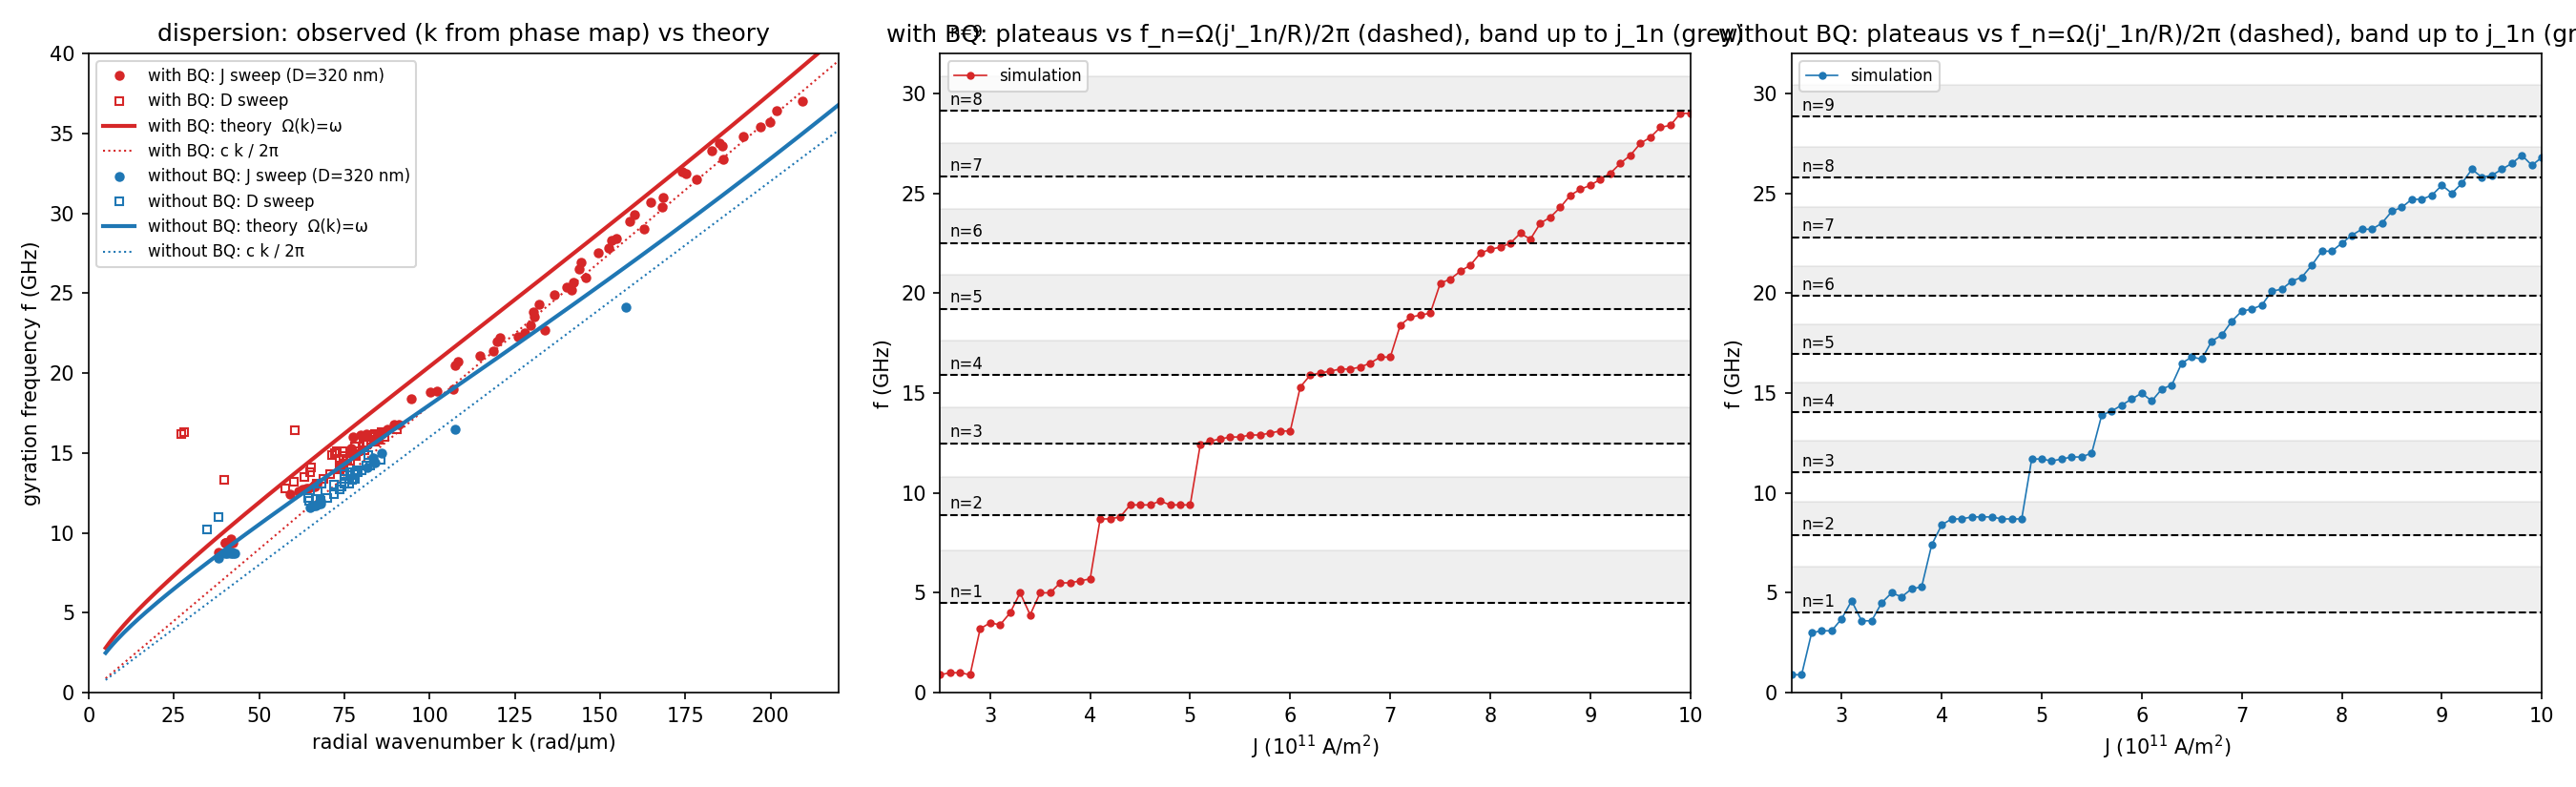
\includegraphics[width=\textwidth]{standing_wave_theory.png}
\caption{Left: simulated gyration frequency versus measured radial wavenumber (circles: $J$ sweep, squares:
$D$ sweep) compared with the selection rule $\Omega(k)=\omega$ from Eq.~\eqref{eq:disp} (solid) and with the
linear limit $ck/2\pi$ (dotted).  Middle and right: simulated frequency versus current density with the
plateau ladder $f_n$ of Eq.~\eqref{eq:ladder} (dashed); the grey bands extend from the free-spin condition
$j'_{1,n}$ to the pinned condition $j_{1,n}$.}
\label{fig:compare}
\end{figure}

\section{Size dependence}
\label{sec:size}

The diameter sweep at fixed current (Supplementary Fig.~1 of the manuscript; $J=6.0$ with BQ and
$5.5\times10^{11}$\,A/m$^2$ without, $D=100$--$700$\,nm in 10\,nm steps) shows three features: a sawtooth in which
the frequency \emph{falls} with diameter and then jumps up, steps that fade above 400--500\,nm, and a slow overall
rise of the frequency.  All three follow from the model, and each was checked against the raw trajectories.
Figure~\ref{fig:size} collects the evidence.

\subsection{The sawtooth: hopping between cavity modes}
Table~\ref{tab:plateaus} lists, for each plateau, the frequency and the directly measured radial phase $kR$ at
its two ends.

\begin{table}[h]
\centering
\caption{Plateaus of the diameter sweep.  $kR$ is measured from the phase maps; $\lambda$ is the wavelength at
the start of the plateau.}
\label{tab:plateaus}
\begin{tabular}{lccccc}
\toprule
 & $D$ (nm) & $f$ (GHz) & $kR$ & width $\Delta D$ (nm) & $\lambda$ (nm)\\
\midrule
with BQ, $n=2$ & 180--240 & $14.8\to12.8$ & $4.9\to6.9$ & 70 & 117\\
\phantom{with BQ, }$n=3$ & 250--320 & $15.0\to13.1$ & $9.0\to10.7$ & 80 & 87\\
\phantom{with BQ, }$n=4$ & 330--390 & $15.0\to14.0$ & $12.7\to14.4$ & 70 & 81\\
\phantom{with BQ, }$n=5$ & 400--460 & $15.1\to14.5$ & $14.9\to17.6$ & 70 & 85\\
\phantom{with BQ, }$n=6$ & 470--520 & $15.4\to15.1$ & $18.4\to20.6$ & 60 & 80\\
\midrule
without BQ, $n=2$ & 180--220 & $12.6\to12.2$ & $6.6\to7.1$ & 50 & 85\\
\phantom{without BQ, }$n=3$ & 230--330 & $14.9\to12.0$ & $9.4\to10.7$ & 110 & 77\\
\phantom{without BQ, }$n=4$ & 340--390 & $13.6\to13.0$ & $13.1\to14.0$ & 60 & 82\\
\bottomrule
\end{tabular}
\end{table}

Three statements can be read off.
\begin{enumerate}
\item \emph{The phase is pinned.}  In the second half of every plateau $kR$ stops growing and stays at a fixed
value $x_n$ ($6.9$, $10.7$, $14.3$, $17.6$, $20.6$ for $n=2\dots6$ with BQ; for instance
$kR=10.63,\,10.75,\,10.64,\,10.69,\,10.70$ for $D=280\dots320$\,nm).  These are the same values found at the plateau
ends of the current sweep (Sec.~\ref{sec:quant}).  With $k=x_n/R$ the selection rule gives
\begin{equation}
f(R)=\frac{1}{2\pi}\,\Omega\!\left(\frac{x_n}{R}\right),
\label{eq:fR}
\end{equation}
a frequency that \emph{decreases} with $R$ because the wave is stretched with the disk.  This is the falling
branch of the sawtooth, and it is the mirror image of the current sweep, where $R$ is fixed and the frequency is
pushed up along the same branch.
\item \emph{Each jump inserts one half wave.}  Across a jump $kR$ increases by about 2\,rad and it gains
another $\simeq1$\,rad while the phase is still free at the beginning of the next plateau, $\pi$ in total.
One more half wave must therefore fit into the radius per plateau, $\Delta R=\lambda/2$, i.e.
\begin{equation}
\Delta D\simeq\lambda ,
\end{equation}
in agreement with the measured widths of 60--80\,nm for $\lambda=80$--$87$\,nm.
\item \emph{The spectral bands are the neighbouring cavity modes.}  The faint lines that run parallel to the
main line in the spin-wave spectra are reproduced by the family $\Omega(j_{1,n}/R)/2\pi$, $n=1,2,\dots$
(dashed curves in Fig.~\ref{fig:size}, top row; no fitted parameter, 4--8\,\% above the simulated plateaus,
which is the known bias of the dispersion).  The oscillator rides on one of these curves and hops to the next.
\end{enumerate}

\subsection{Why the frequency follows the wave: power balance}
\label{sec:power}
What decides the frequency, and why the cavity can pull it, follows from an exact identity of the LLG equation.
Write the conservative field as $\vect H_c$ and the spin torque as in Eq.~\eqref{eq:stt}:
$\partial_t\vect m=-\gamma\,\vect m\times\vect H_c-\gamma a_J\,\vect m\times(\vect m\times\vect p)
+\alpha\,\vect m\times\partial_t\vect m$.
Taking the cross product with $\vect m$ and using $\vect m\times(\vect m\times\vect v)=-\vect v$ for any
$\vect v\perp\vect m$,
\begin{equation}
\vect m\times\partial_t\vect m=\gamma\big[\vect H_c-(\vect m\cdot\vect H_c)\vect m\big]
+\gamma a_J\,\vect m\times\vect p-\alpha\,\partial_t\vect m .
\end{equation}
The scalar product with $\partial_t\vect m$ (which is perpendicular to both $\vect m$ and
$\vect m\times\partial_t\vect m$) gives
\begin{equation}
\alpha\,|\partial_t\vect m|^2=\gamma\,\vect H_c\cdot\partial_t\vect m
+\gamma a_J\,(\vect m\times\vect p)\cdot\partial_t\vect m .
\end{equation}
Integrated over the layer, $\mu_0\Ms\int\vect H_c\cdot\partial_t\vect m\,\dd V=-\dd E/\dd t$, which averages to
zero in a steady state.  With $\vect p=\uv z$, $(\vect m\times\vect p)\cdot\partial_t\vect m
=-(\vect m\times\partial_t\vect m)_z$, so that
\begin{equation}
\boxed{\;\alpha\,\big\langle|\partial_t\vect m|^2\big\rangle
=\gamma a_J\,\big\langle-(\vect m\times\partial_t\vect m)_z\big\rangle\;}
\label{eq:power}
\end{equation}
(space and time average): Gilbert dissipation equals the work done by the spin torque.  For the rigid rotation
of Sec.~\ref{sec:macrospin} both sides are proportional to $\cos^2\theta_0$ and Eq.~\eqref{eq:power} reduces to
$\alpha\omega=\gamma a_J$, i.e.\ to the macrospin frequency
\begin{equation}
f_\mathrm{mac}=\frac{\gamma a_J}{2\pi\alpha},\qquad a_J=\frac{\hbar JP}{2e\mu_0\Ms d},
\end{equation}
which is 20.5\,GHz at $J=6.0$ and 18.8\,GHz at $J=5.5\times10^{11}$\,A/m$^2$.
Note that $f_\mathrm{mac}$ does not depend on the biquadratic coupling; the coupling changes the tilt, not the
balance.

In the disk the magnetisation is the rigid rotation plus the wave.  Using the spin-frame decomposition
$\partial_t\vect m=\mathsf R_z(\partial_t\vect m'+\dot\Phi\,\uv z\times\vect m')$,
\begin{align}
|\partial_t\vect m|^2&=\dot\Phi^2m_\parallel^2+|\partial_t\vect m'|^2+2\dot\Phi\,(\vect m'\times\partial_t\vect m')_z,\\
(\vect m\times\partial_t\vect m)_z&=\dot\Phi\,m_\parallel^2+(\vect m'\times\partial_t\vect m')_z,
\end{align}
with $m_\parallel^2=m_x^2+m_y^2$.  Defining the two dimensionless wave quantities
\begin{equation}
s=\frac{\langle|\partial_t\vect m'|^2\rangle}{\omega^2\langle m_\parallel^2\rangle},\qquad
x=\frac{\langle(\vect m'\times\partial_t\vect m')_z\rangle}{\dot\Phi\,\langle m_\parallel^2\rangle},
\end{equation}
Eq.~\eqref{eq:power} becomes
\begin{equation}
\frac{f}{f_\mathrm{mac}}=\eta\,\frac{1+x}{1+s+2x},
\label{eq:fratio}
\end{equation}
where $\eta$ is unity if Eq.~\eqref{eq:power} closes within the free layer alone.  All three factors were
evaluated from the last 3\,ns of each of the 122 runs of the diameter sweep (\texttt{power\_balance.py}).
The result is $1+x=0.87$--$0.90$, almost independent of diameter; $\eta=0.80$--$0.86$, also nearly constant
(see Sec.~\ref{sec:limits} for this deficit); and an excess-dissipation factor $1+s+2x$ that carries the size
dependence, from $0.96$ in the largest disks to $1.10$--$1.14$ at the ends of the first plateaus.  For example,
at $D=320$\,nm with BQ, $0.80\times0.88/1.098=0.64$, against $13.1/20.5=0.64$; at $D=700$\,nm,
$0.85\times0.90/0.961=0.80$, against $16.3/20.5=0.80$.

\subsection{An empirical law: frequency versus wave power}
The wave content can be condensed into a single number: the mean-square in-plane amplitude at the gyration
frequency in the co-rotating spin frame,
\begin{equation}
\langle a^2\rangle=\Big\langle\,\big|m'_+(\vect r,t)\big|^2_{\,0.5\omega<|\Omega|<1.5\omega}\Big\rangle ,
\end{equation}
which is the power in the phase component $a$ of the wave of Sec.~\ref{sec:disp} (the out-of-plane component is
about 13 times weaker in power; the linear theory gives the ellipticity $N_{22}/N_{11}\simeq14$--$18$).  Plotted
against $\langle a^2\rangle$, the frequencies of all runs with $D=180$--$700$\,nm fall on a single curve for
each coupling (Fig.~\ref{fig:size}, bottom),
\begin{equation}
\boxed{\;f=\frac{f_\mathrm{mac}}{1+\beta\,\langle a^2\rangle}\;},\qquad
\beta=2.2\ \text{(BQ)},\quad 2.6\ \text{(no BQ)},
\label{eq:collapse}
\end{equation}
with an rms residual of 0.4\,GHz and a correlation of $-0.88$ (BQ) and $-0.84$ (no BQ) between $f$ and
$\langle a^2\rangle$.  Here $f_\mathrm{mac}$ is the calculated macrospin value and $\beta$ is the only fitted
constant.  Equation~\eqref{eq:collapse} is the quantitative form of the statement in the supplementary material
that energy diverted into the spin wave lowers the frequency.
It is not a consequence of Eq.~\eqref{eq:fratio}.  With no wave ($s=x=0$) that equation gives $f/f_\mathrm{mac}=\eta
\approx0.8$, whereas Eq.~\eqref{eq:collapse} is pinned to $f=f_\mathrm{mac}$ at $\langle a^2\rangle=0$, and the
relation between $1+s+2x$ and $\langle a^2\rangle$ has not been derived.  The two are linked only qualitatively,
and the unidentified deficit $\eta$ (Sec.~\ref{sec:limits}) is where they meet.  The same law holds in the current
sweep with $\beta=2.4$ (BQ) and $2.6$ (no BQ) and an rms residual of 0.04\,GHz, against 0.4\,GHz
for the diameter sweep here.

\subsection{The feedback that pins the phase}
Equations \eqref{eq:selection}, \eqref{eq:collapse} and the cavity response close a loop:
\begin{center}
$f\ \xrightarrow{\ \Omega(k^\ast)=\omega\ }\ k^\ast\ \longrightarrow\ k^\ast R\ \xrightarrow{\ \text{cavity}\ }\
\langle a^2\rangle\ \xrightarrow{\ \text{Eq.~\eqref{eq:collapse}}\ }\ f .$
\end{center}
Just after a jump the phase $k^\ast R$ is on the low side of the $n$-th resonance, the wave is weak
($\langle a^2\rangle\simeq0.11$--$0.17$) and the oscillator runs at its upper frequency (15\,GHz with BQ,
13.6--13.9\,GHz without, for $D\le400$\,nm).  As the disk grows, $k^\ast R$ moves towards the resonance and the
wave grows; the frequency drops, and with it $k^\ast$, so that $k^\ast R$ advances more slowly than $R$ and finally
not at all.  This negative feedback is the pinning of item~1 above.  The wave power reaches
$\langle a^2\rangle\simeq0.23$--$0.26$ at the end of a plateau and falls by 30--40\,\% at the jump (third row of
Fig.~\ref{fig:size}), when the rim drive can no longer sustain the stretched pattern and the next mode, which
fits with a weaker wave, takes over.

\subsection{Fading of the steps and the slow rise}
The cavity exists only if the inward wave returns from the centre.  The wave is damped at the rate
$\Gamma=\alpha\gamma(N_{11}+N_{22})/2$ and travels at the group velocity $v_g=\partial\Omega/\partial k$, so its
amplitude decays over
\begin{equation}
\ell=\frac{v_g}{\Gamma}=\frac{2}{\alpha\gamma}\,\frac{\partial\Omega/\partial k}{N_{11}+N_{22}}
\simeq173\ \mathrm{nm}\ \text{(BQ, 16\,GHz)},\qquad 193\ \mathrm{nm}\ \text{(no BQ, 14.8\,GHz)},
\label{eq:ell}
\end{equation}
with $v_g=1141$ and $1022$\,m/s and $\Gamma=6.6$ and $5.3\ \mathrm{ns}^{-1}$.  Fitting the radial envelope of the
maps in the largest disks, after removing the geometric $r^{-1/2}$ focusing, gives $114,\ 153,\ 167$\,nm
($D=500,\ 600,\ 700$\,nm, BQ) and $94,\ 136,\ 191$\,nm (no BQ), consistent with Eq.~\eqref{eq:ell}.
The amplitude that survives a round trip is $\ee^{-2R/\ell}$: about 15\,\% at $D=320$\,nm, 5\,\% at 500\,nm and
2\,\% at 700\,nm.  Beyond $D\simeq400$--$500$\,nm there is therefore no standing wave to speak of, the cavity
resonances disappear and the sawtooth dies out, as observed.  Without BQ the large disks are in addition far less
phase-coherent (the magnitude of the spatially averaged in-plane moment is 0.2--0.5, against 0.7--0.8 with BQ),
which washes the pattern out earlier.

The slow rise has the same origin.  The wave is launched at the rim and fills a strip of width $\sim\ell$, so the
area-averaged wave power falls roughly as $1/R$ once $R>\ell$: $\langle a^2\rangle=0.15$ at 500\,nm and $0.12$
at 700\,nm with BQ.  By Eq.~\eqref{eq:collapse} the frequency keeps creeping up, from 15.4 to 16.3\,GHz over that
range.  The apparent saturation above 500\,nm is thus a slow approach towards $f_\mathrm{mac}$, not a true
plateau.

\begin{figure}[p]
\centering
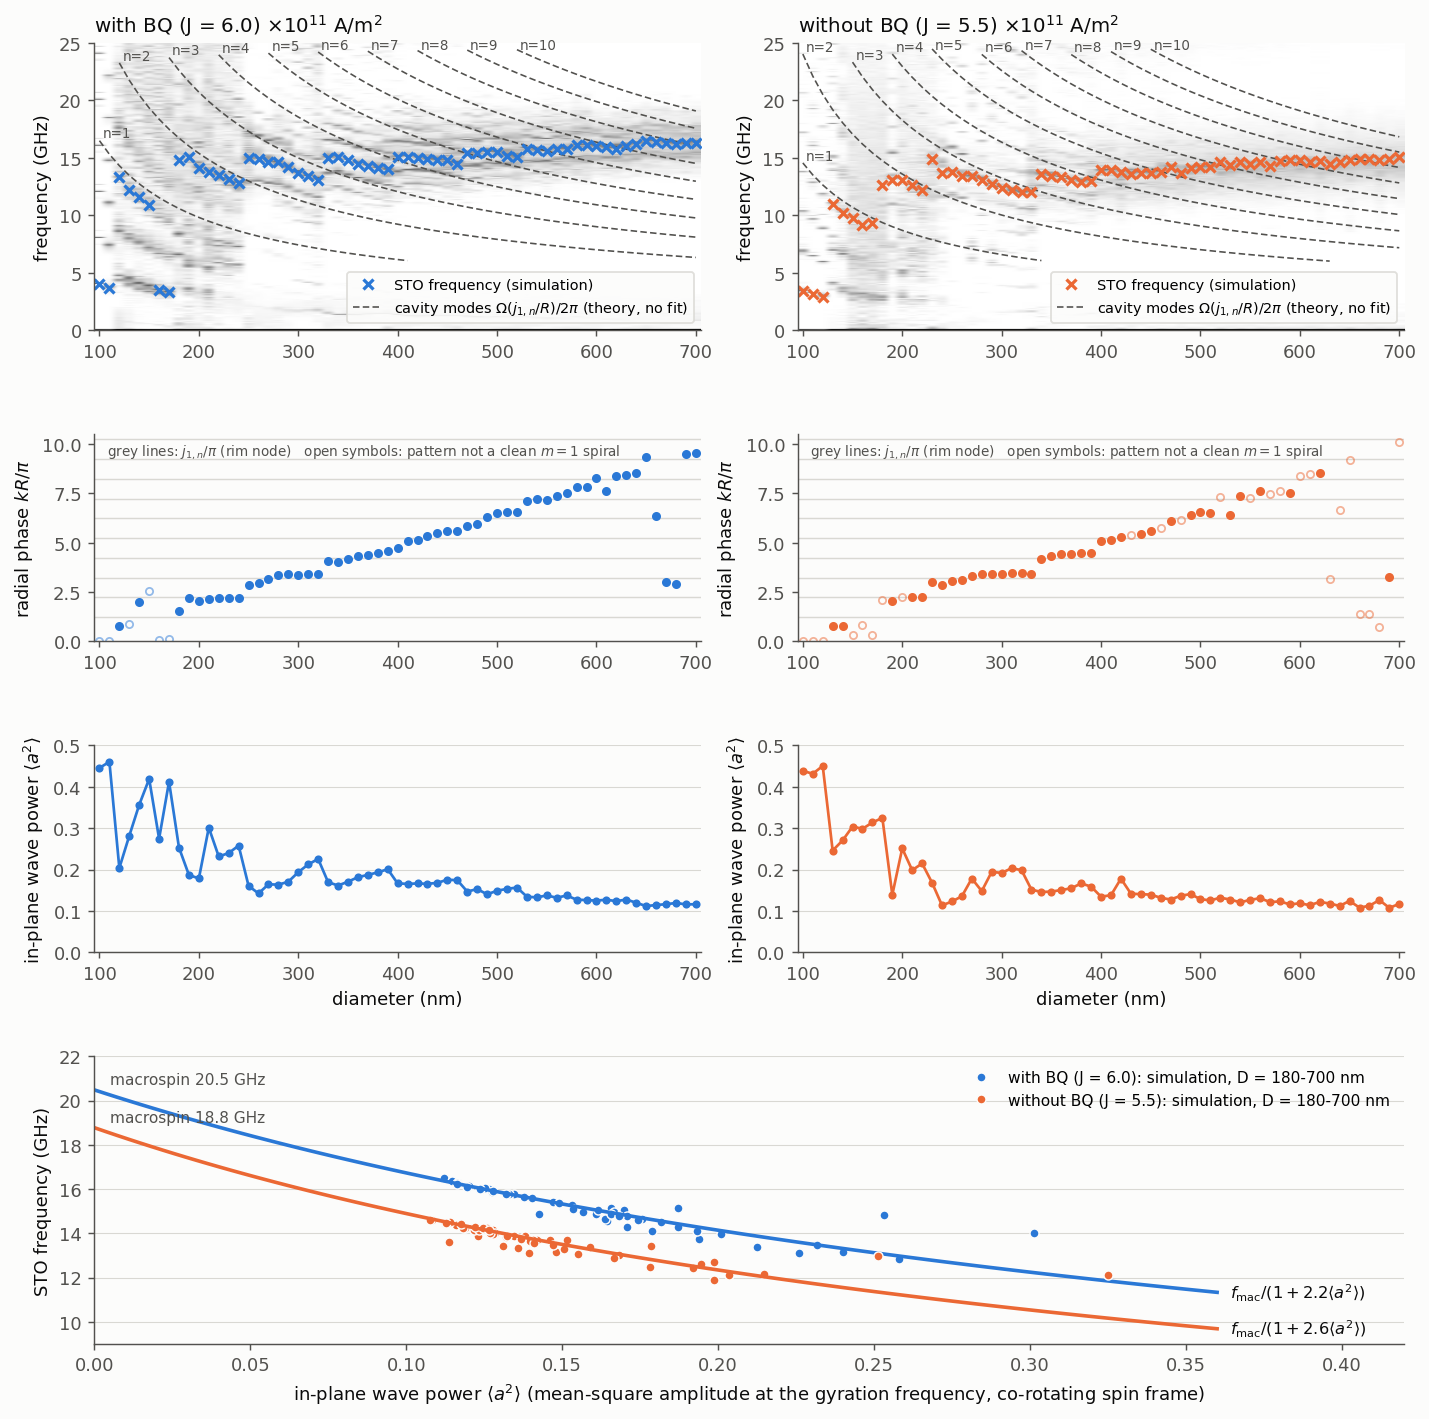
\includegraphics[width=\textwidth]{size_dependence.png}
\caption{Size dependence, with BQ (left, blue) and without (right, orange).  First row: spin-wave spectra of the
diameter sweep (grey scale), frequency of the average in-plane magnetisation (crosses) and the cavity-mode family
$\Omega(j_{1,n}/R)/2\pi$ (dashed, no fit).  Second row: radial phase $kR/\pi$ measured from the phase maps; the
grey lines mark $j_{1,n}/\pi$.  Third row: in-plane wave power $\langle a^2\rangle$.  Bottom: frequency versus
wave power for all runs with $D\ge180$\,nm and the one-parameter law of Eq.~\eqref{eq:collapse}.}
\label{fig:size}
\end{figure}

\subsection{What is not explained}
For $D<180$\,nm the model does not apply.  The states at 3--5\,GHz ($D=100,\ 110,\ 160,\ 170$\,nm with BQ,
$100$--$120$\,nm without) are not a coherent gyration: their dissipation is three to six times that of a rigid
rotation and most of it sits at frequencies far above the gyration.  Between them the $n=1$ cavity branch appears
($D=120$--$150$\,nm with BQ, $130$--$170$\,nm without) and follows the $n=1$ curve.

\section{Approximations, and what the model does not give}
\label{sec:limits}
\begin{itemize}
\item The dipolar orientation factors were averaged over the azimuth, the film is treated as infinite in-plane
for the dispersion, and the linearisation is used at a wave amplitude of $\delta m_z\simeq0.17$.  The systematic
$+7\,\%$ of $f_\mathrm{theory}/f_\mathrm{sim}$ is of the size expected from these approximations.  A full
treatment would solve the linearised problem numerically on the disk with the exact demagnetising kernel.
\item The rim is a driven, textured region about 15\,nm wide, so the effective cavity radius and the edge phase
are uncertain at the 10\,\% level; the grey bands in Fig.~\ref{fig:compare} bracket this uncertainty, and the
directly measured phases lie at or slightly beyond their upper edge (Sec.~\ref{sec:quant}).
\item The absolute frequency is tied to the wave power by the exact balance \eqref{eq:power} and, empirically, by
Eq.~\eqref{eq:collapse}, but the wave power itself (the response of the driven cavity to the rim field, including
its nonlinear saturation) is taken from the simulation; it is not derived.  The constant $\beta$ is fitted.
\item The balance \eqref{eq:power} closes only to $\eta=0.80$--$0.86$ when the dissipation is evaluated in the free
layer alone.  Of the deficit, 3--5\,\% is the finite-difference time derivative on the 5\,ps output grid; the
remainder is nearly independent of diameter and of the coupling and has not been identified (the fixed layer is
dynamic, with $\alpha=0.1$, and is a candidate).  It does not affect the size dependence.
\item The in-plane anisotropy (3.5\,mT) and the $0.6^\circ$ polariser tilt were neglected.  In the rotating
frame they act as weak drives at $2\omega$ ($m=0$) and at $\omega$ ($m=0$), respectively; they are responsible for
the small counter-rotating and $m=0$ admixtures observed in the raw data.
\end{itemize}

\appendix
\section{Thin-film dipolar tensor}
For a film of thickness $d$ with in-plane wavevector $\vect k$ and a magnetisation uniform across the thickness,
the thickness-averaged demagnetising tensor is
$\mathsf N(\vect k)=P(kd)\,\uv z\uv z^{\mathsf T}+\big(1-P(kd)\big)\,\uv k\uv k^{\mathsf T}$,
$P(x)=(1-\ee^{-x})/x$, which reduces to $\uv z\uv z^{\mathsf T}$ at $k=0$ and to $\uv k\uv k^{\mathsf T}$ for
$kd\to\infty$ (bulk).  Equation~\eqref{eq:dip} is $\delta\vect H_\mathrm{d}=-\Ms\mathsf N(\vect k)\delta\vect m$.

\section{Bessel zeros used}
$j_{1,n}$ (zeros of $J_1$): 3.832, 7.016, 10.173, 13.324, 16.471, 19.616, 22.760.\\
$j'_{1,n}$ (zeros of $J_1'$): 1.841, 5.331, 8.536, 11.706, 14.864, 18.016, 21.164, 24.311.

\section{Numerical values}
\begin{tabular}{p{0.42\textwidth}p{0.52\textwidth}}
$D=2A/\mu_0\Ms$ & $1.533\times10^{-11}$\,A\,m\\
$\HB=2|B_{12}|/\mu_0\Ms d$ & $3.54\times10^{5}$\,A/m ($\mu_0\HB=0.444$\,T)\\
$\gamma/2\pi$ & 28.0\,GHz/T\\
$c=\gamma\sqrt{D\Ms}$, $\gamma\sqrt{D(\Ms+\HB)}$ & 1006, 1130\,m/s\\
$m_{z0}$ at 13.1\,GHz (BQ), 12.0\,GHz (no BQ) & 0.22, 0.25 (simulated 0.26, 0.28)\\
$k^\ast$ at $D=320$\,nm, BQ / no BQ & 67 / 68\,$\mu$m$^{-1}$ (phase slope), 70\,$\mu$m$^{-1}$ (node positions)\\
\end{tabular}

\section{Files}
\begin{tabular}{p{0.26\textwidth}p{0.68\textwidth}}
\texttt{wave\_extract.py} & azimuthal decomposition of all FFT maps, writes \texttt{wave\_table.csv}\\
\texttt{sw\_theory.py} & Eqs.~\eqref{eq:disp}, \eqref{eq:selection}, \eqref{eq:ladder}; makes \texttt{standing\_wave\_theory.png}\\
\texttt{frame\_check.py} & raw-data checks (gyration sense, tilt, harmonics), results in \texttt{frame\_check\_results\_raw.txt}\\
\texttt{power\_balance.py} & exact power balance and wave power for the diameter sweep, writes \texttt{power\_balance.csv}\\
\texttt{size\_dependence.py} & Sec.~\ref{sec:size}; makes \texttt{size\_dependence.png}\\
\end{tabular}

Note on conventions: magnum.np stores arrays as \texttt{[x, y, z, component]}; a script that interprets the first
index as $y$ mirrors the image and flips the sign of the azimuthal index.

\end{document}
